% arara: pdflatex: { synctex: yes }
% arara: makeindex: { style: ctuthesis }
% arara: bibtex

% The class takes all the key=value arguments that \ctusetup does,
% and a couple more: draft and oneside
\documentclass[twoside]{ctuthesis}

\ctusetup{
	preprint = \ctuverlog,
	mainlanguage = english,
	titlelanguage = english,
%	mainlanguage = czech,
	otherlanguages = {czech,english},
	title-czech = {Rádiové určování polohy letících objektů},
	title-english = {Radio position determination of the flying objects},
%	subtitle-czech = {Cesta do tajů kdovíčeho},
%	subtitle-english = {Journey to the who-knows-what wondeland},
	doctype = D,
	doctype-czech = Obhajoba minima,
    doctype-english = Thesis proposal, % or whatever
	faculty = F3,
	department-czech = {Katedra měření},
	department-english = {Department of Measurement},
	author = {Jakub Kákona},
	supervisor = {Doc. Dr. Ing. Pavel Kovář},
	supervisor-address = {Department of Radio Engineering, \\ Uliční 5, \\ Praha 99},
%	supervisor-specialist = {John Doe},
	fieldofstudy-english = {Air Traffic Control},
	subfieldofstudy-english = {Radio navigation},
	fieldofstudy-czech = {Provoz a řízení letecké dopravy},
	subfieldofstudy-czech = {Rádiová navigace},
	keywords-czech = {slovo, klíč},
	keywords-english = {word, key},
	day = 27,
	month = 11,
	year = 2016,
%	specification-file = {ctutest-zadani.pdf},
%	front-specification = true,
%	front-list-of-figures = false,
%	front-list-of-tables = false,
%	monochrome = true,
%	layout-short = true,
%	savetoner = true,
}

\ctuprocess

\addto\ctucaptionsczech{%
	\def\supervisorname{Vedoucí}%
	\def\subfieldofstudyname{Studijní program}%
}

\ctutemplateset{maketitle twocolumn default}{
	\begin{twocolumnfrontmatterpage}
%		\ctutemplate{twocolumn.thanks}
%		\ctutemplate{twocolumn.declaration}
		\ctutemplate{twocolumn.abstract.in.titlelanguage}
		\ctutemplate{twocolumn.abstract.in.secondlanguage}
		\ctutemplate{twocolumn.tableofcontents}
		\ctutemplate{twocolumn.listoffigures}
	\end{twocolumnfrontmatterpage}
}

% Theorem declarations, this is the reasonable default, anybody can do what they wish.
% If you prefer theorems in italics rather than slanted, use \theoremstyle{plainit}
\theoremstyle{plain}
\newtheorem{theorem}{Theorem}[chapter]
\newtheorem{corollary}[theorem]{Corollary}
\newtheorem{lemma}[theorem]{Lemma}
\newtheorem{proposition}[theorem]{Proposition}

\theoremstyle{definition}
\newtheorem{definition}[theorem]{Definition}
\newtheorem{example}[theorem]{Example}
\newtheorem{conjecture}[theorem]{Conjecture}

\theoremstyle{note}
\newtheorem*{remark*}{Remark}
\newtheorem{remark}[theorem]{Remark}

\setlength{\parskip}{5ex plus 0.2ex minus 0.2ex}


% Only for testing purposes
\listfiles
\usepackage[pagewise]{lineno}
\usepackage{lipsum,blindtext}
\usepackage{mathrsfs} % provides \mathscr used in the ridiculous examples

\begin{document}

\maketitle

\chapter{Motivation}

Radio position determination of flying objects is standard radio location discipline which led to development of RADAR systems. At the present time the RADAR systems are enough mature to detect almost any radio-reflective artificial flying object in atmosphere or in near space. Therefore technology development is moving from focus on RADAR sensitivity to system stability, reliability and low operation costs. Resulting applied technologies leads to new scientific possibilities of observations and measurement which could bring new discoveries. 

\section{Flying object parameters}

From radar point of view where terminology usually uses a term target instead of object. The radar cross section (RCS) and object velocity are limiting parameters of the radar systems. These parameters vary largely depending on measured flying object type. 

\subsection{Artificial airspace targets}

A large group of possible radio reflective targets are classical airspace objects as airplanes, Unmanned Aerial vehicles or satellites. These classical objects are usually detectable and localizable with already existing radar systems. Parameters like RCS and trajectory or velocity of these object is also known. Therefore this object category could be used for new system verification. 

\subsection{Natural radio-detectable objects}

Several natural atmospheric or near space phenomena are expected to be localized by radio-waves. The list contains Solar system bodies, meteors, ionospheric fluctuations, cosmic rays particles and atmospheric electrical discharges. Not all of these natural phenomenons have confirmed radio detection due to technical or yet unknown physical principles. But observation of natural phenomenons are generally scientifically more valuable than artificial objects. Therefore the work will be mainly focused on methods useful of natural phenomena measurement and detection. 

Meteors were selected as primary testing phenomenon because they have unusual special properties like high velocities and wide range of RCS. Meteors, the products of meteoroids travelling in space, are studied for many decades. Results of such research help us to understand the evolution of not only the planetary system but the interplanetary medium \cite{interplanetary_medium} as well. As the density of the interplanetary medium is low, large statistical and long term continuous data set is necessary to describe its properties. There exist two radio waves observation methods which use the scattering ability of the ionized meteor trail.

The oldest known radio method is a backscatter radar. It is an ordinary type of radar which expects meteor trails to be reflective targets. Currently, several radars of this type are in operation to study meteors i. e.  SkiYMet\cite{skiymet}, CMOR \cite{CMOR_radar}.

The general principle of meteor observing by the forward scattering of radio waves off their trails is illustrated in figure \ref{fig:forward_scattering}. A radio receiver with operating frequency range of 30-200MHz is located at proper distance (about 500-2000 km) from a transmitter. A curvature of the Earth over this distance ensures no possibility of direct radio wave contact. When a meteoroid enters the atmosphere, its meteor trail may reflect the radio waves emitted by transmitter to the receiver. The signal can be received until the ionized meteor trail recombines. Reflections can last from a tenths of a second to a few minutes, depending on their frequency and ionization intensity. The received signal characteristics are related to physical parameters of the meteoric event \cite{forward_scatter}.

However, all of above mentioned monostatic or bistatic radars have very small detection coverage, usually limited to the radar antenna field of view. Therefore this radar types observe only several spatially limited areas of the Earth's atmosphere. But the benefits of using this method are obvious - radio meteor detection capability is not dependent on the current weather and can work even during the daylight or nights with full Moon \cite{daylight_shover}.

Besides the above-mentioned scientific radar systems a multistatic radio meteor detection networks have evolved \cite{BRAMS}.
These forward scattering multistatic systems have great advantage of a large detection coverage. Unfortunately, the current spread of this technology is not sufficient to entirely cover the meteor flux of the Earth's atmosphere.


\begin{figure}
 \begin{center}
 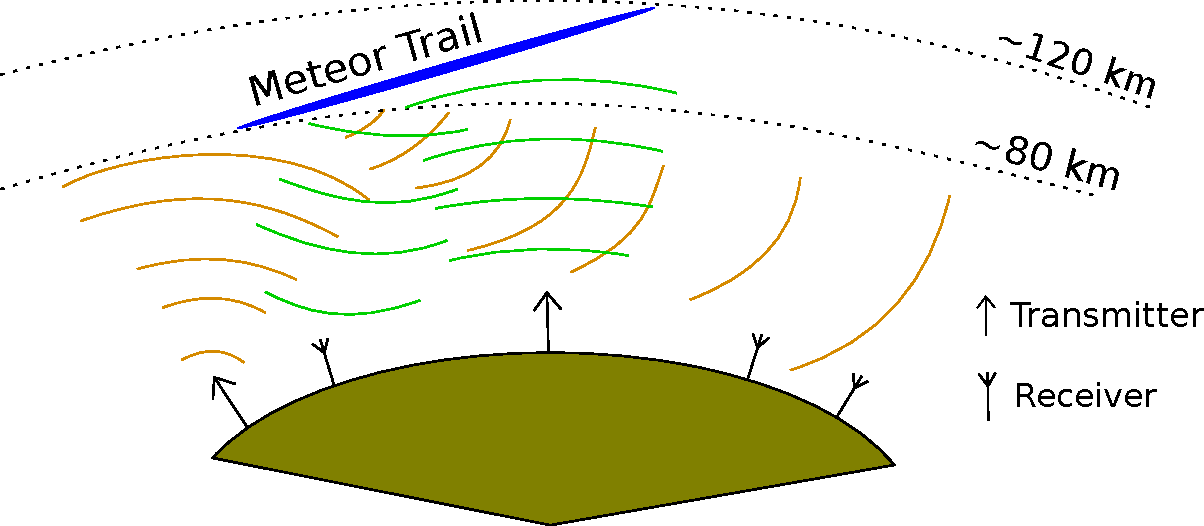
\includegraphics[width=\linewidth]{./img/Meteor_detection.pdf}
 \caption{The method of radio meteor detection based on the forward scattering radar system}
  \label{fig:forward_scattering} 
 \end{center}
\end{figure}

\subsection{Position determination methods}

If we want to find out object position by radio signal reflected or transmitted by the object. We have only a small number of signal features which we could use to obtain information about object coordinates. The best method used for determination of object position depends on type of an object required precision of measurement and application. In most cases for unknown flying object we need to combine several of following methods. 

\subsection{Triangulation}

Radio direction finding is the oldest radio localization method. 

\subsection{Distance measurement}


\subsection{Velocity measurement}


The key principle is bistatic Doppler shift described by equation \ref{bistatic_doppler}. 

\begin{equation}
f = \frac{1}{\lambda} \frac{d}{dt} \left( R_{tx} + R_{rx} \right)
\label{bistatic_doppler}
\end{equation}

Where 
\begin{itemize}
\item $f$ - Received frequency
\item $\lambda$ - Radar transmitter operating frequency wavelength in meters
\item $R_{tx}$ - Distance between transmitter and target
\item $R_{rx}$ - Distance between receiver and target.
\end{itemize}

\chapter{Meteor trajectory determination}

Every radio illuminated meteor trajectory in atmosphere create its own Doppler shift reflection footprint.  This process could be easily modeled by a numerical calculation of Doppler shifts in points of trajectory. For a simplicity, the presented model expects constant velocity along a straight line of the meteor path which is divided to equidistant time samples. A numerical difference of path distances between transmitter, meteor and receiver is calculated. Then velocity and Doppler shift value is obtained for every point of trajectory. 
The resulting figure of Doppler shifts calculated along the model meteor path visible to every existing station is shown in figure \ref{fig:dopplers}. 


\begin{figure*}
 \begin{center}
 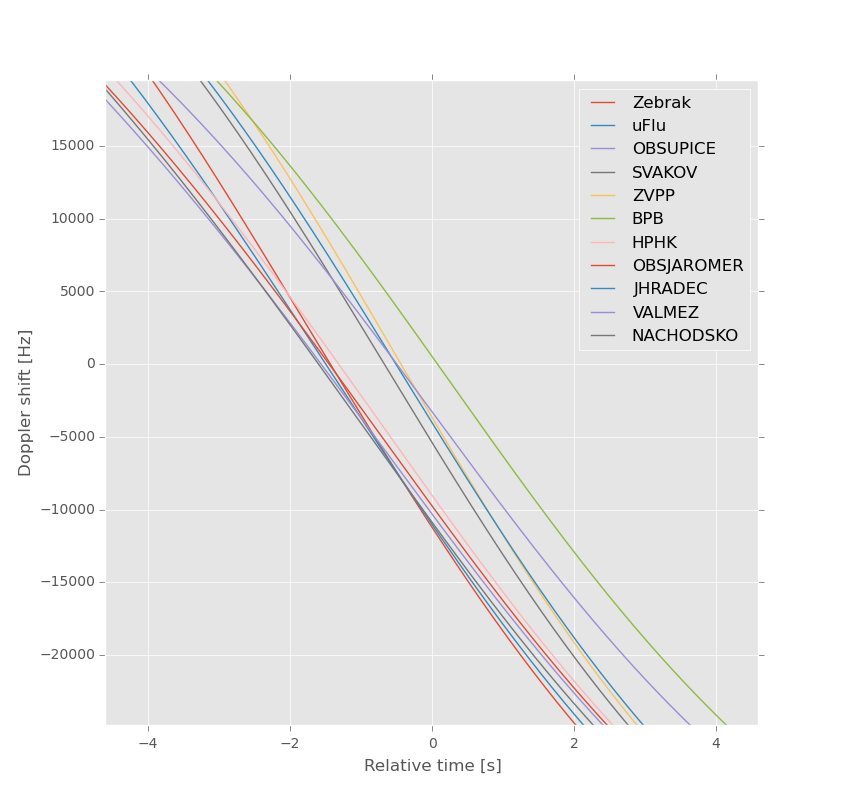
\includegraphics[width=\textwidth]{./img/Meteor_dopplers.png}
 \caption{Doppler shifts calculated for meteor ground path displayed in the figure \ref{fig:stanice_mapa}.}
  \label{fig:dopplers} 
 \end{center}
\end{figure*}


This signal model can be easily confirmed from meteor database where several meteor events are detected on multiple stations. If we plot such meteor event in time aligned spectrogram we obtain an image similar to the figure \ref{fig:meteor_reflections}.
Precise meteor trajectory estimation methods are intensively investigated at the moment.  One of the difficulties is a suboptimal geometry situation and low inter-station events correlation. Therefore expanding of the network is another task which runs in parallel. 


\section{GRAVES based detection system}

Bolidozor uses multistatic forward scattering approach which allows an efficient use of the radar transmitter energy  to maximize the information value collected from the meteor reflection.
The network currently uses GRAVES \cite{GRAVES_radar} transmitter located in France, which transmits a CW (continuous wave) signal at a frequency of 143.05 MHz. A radiation of the transmitter is directed mainly to the south hemisphere, but due to the imperfections of its antenna system, the signal from meteor reflections can be observed in almost all European countries. Therefore the transmitter is suitable for receivers' network operations with the aim of meteor trail detection and the development of algorithms for the calculation of meteor trajectory.

\begin{figure}
 \begin{center}
 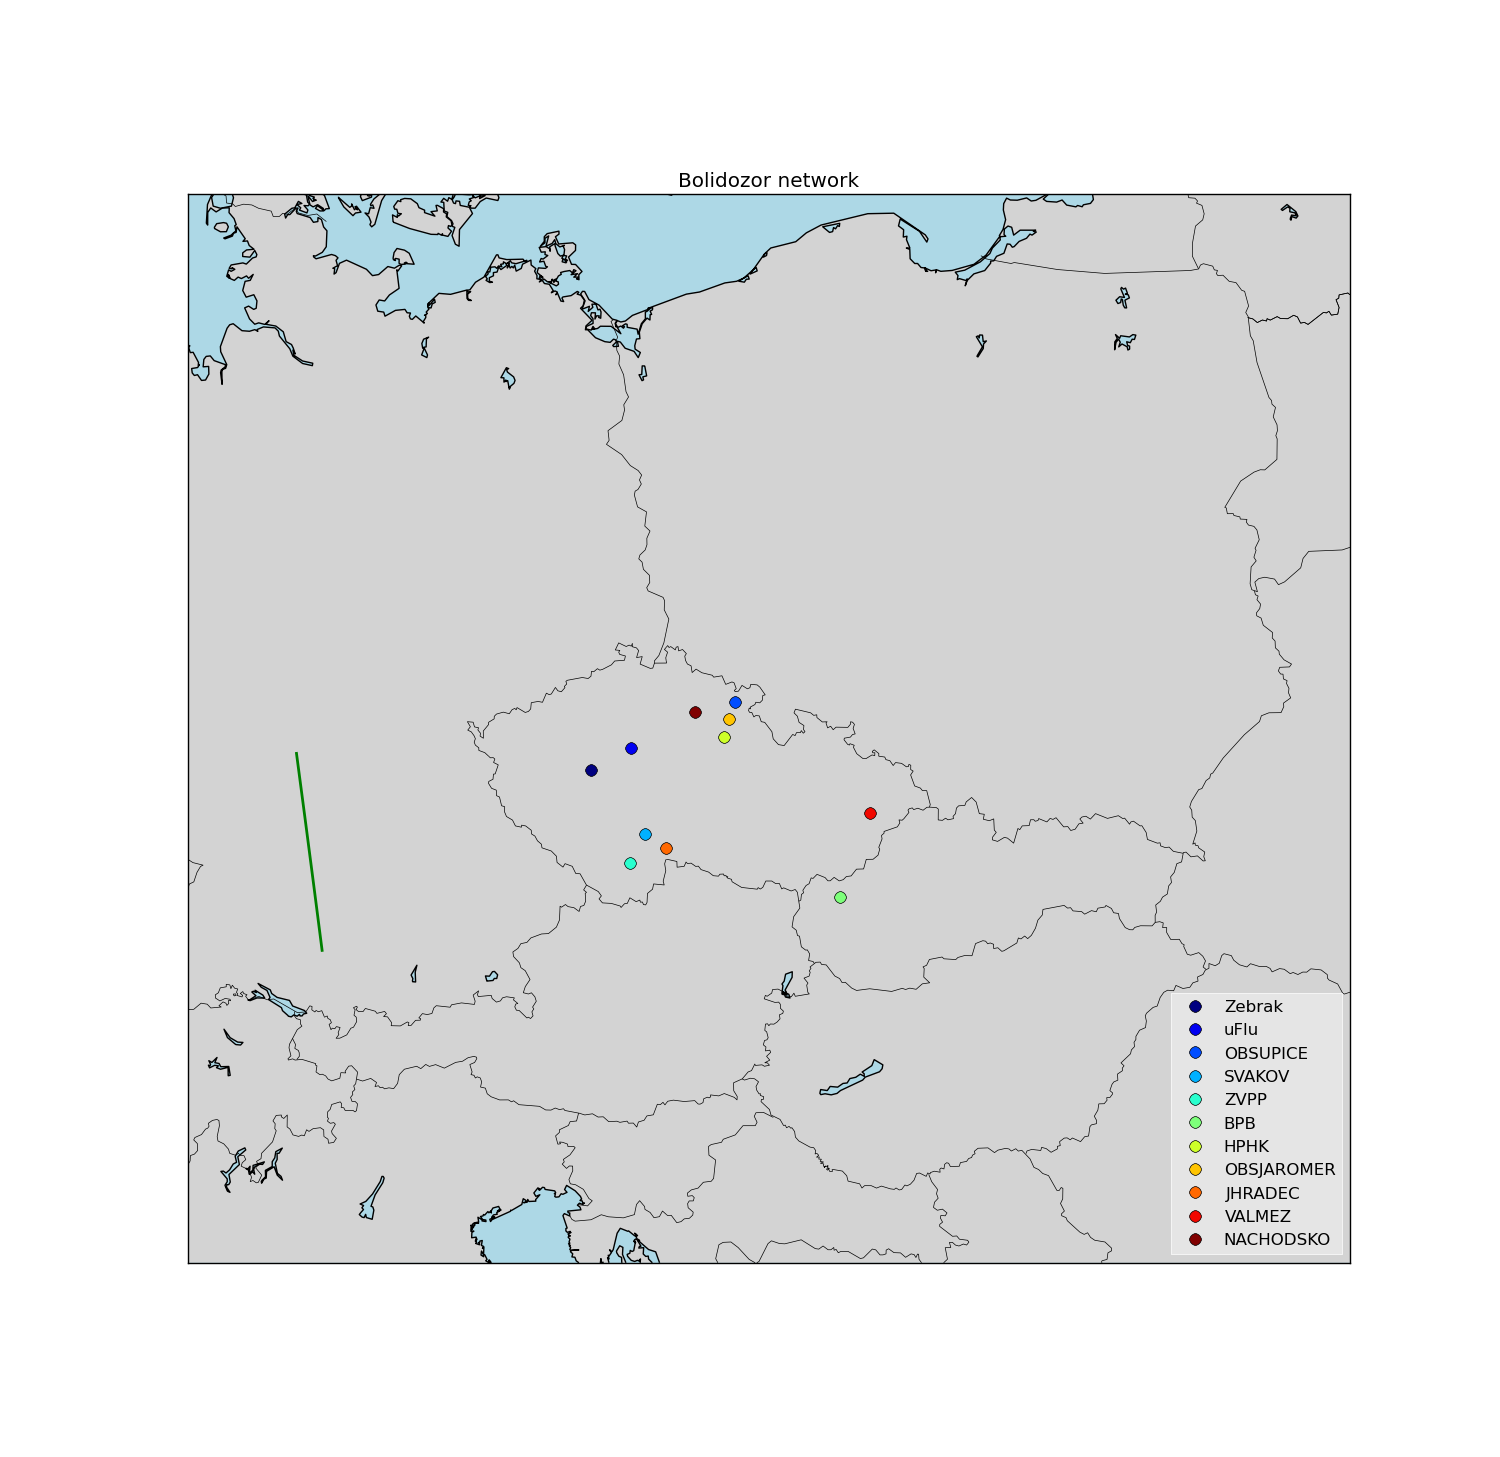
\includegraphics[width=\linewidth]{./img/stanice_mapa.png}
 \caption{Bolidozor stations network}
  \label{fig:stanice_mapa} 
 \end{center}
\end{figure}
                   
The use of such high frequency beacon has one main advantage over the previous experiments.
Previous attempts used longer wavelengths in frequency range 20-50 MHz. Such long wavelengths were used to obtain a higher sensitivity to finer meteor trails. According to a simplified formula (\ref{equ:decay}), where $T$ is exponential time constant and $D$ is ambipolar diffusion coefficient and $\lambda$ is wavelength \cite{Decay_time}, we have longer meteor echos from meteors with the same ionisation energy observed by longer wavelengths compared to meteor reflections observed by shorter wavelengths. But shorter wavelengths allow us to detect finer details of meteor trails.

\begin{equation}
T = \frac{\lambda^2}{16 \pi ^2 D}
\label{equ:decay}
\end{equation}

The head echo of meteor is usually called as overdense due to its relatively high plasma frequency compared to used observation frequency ($F_{obs}$) in the front of the meteoroid shock wave that is created in the air. This condition is expressed by the equation (\ref{equ:plasma_frequency}). However, if we use a frequency near to the plasma frequency ($f_{pe}$) of the meteor trail we can distinguish the head echo and meteor trail reflection because the Doppler shift is applied on the part of reflected signal. This situation is shown in the figure \ref{fig:meteor_reflections} where head echoes are marked by sloped dotted lines. Static meteor trail reflections are marked by straight vertical lines.

\begin{figure*}
 \begin{center}
 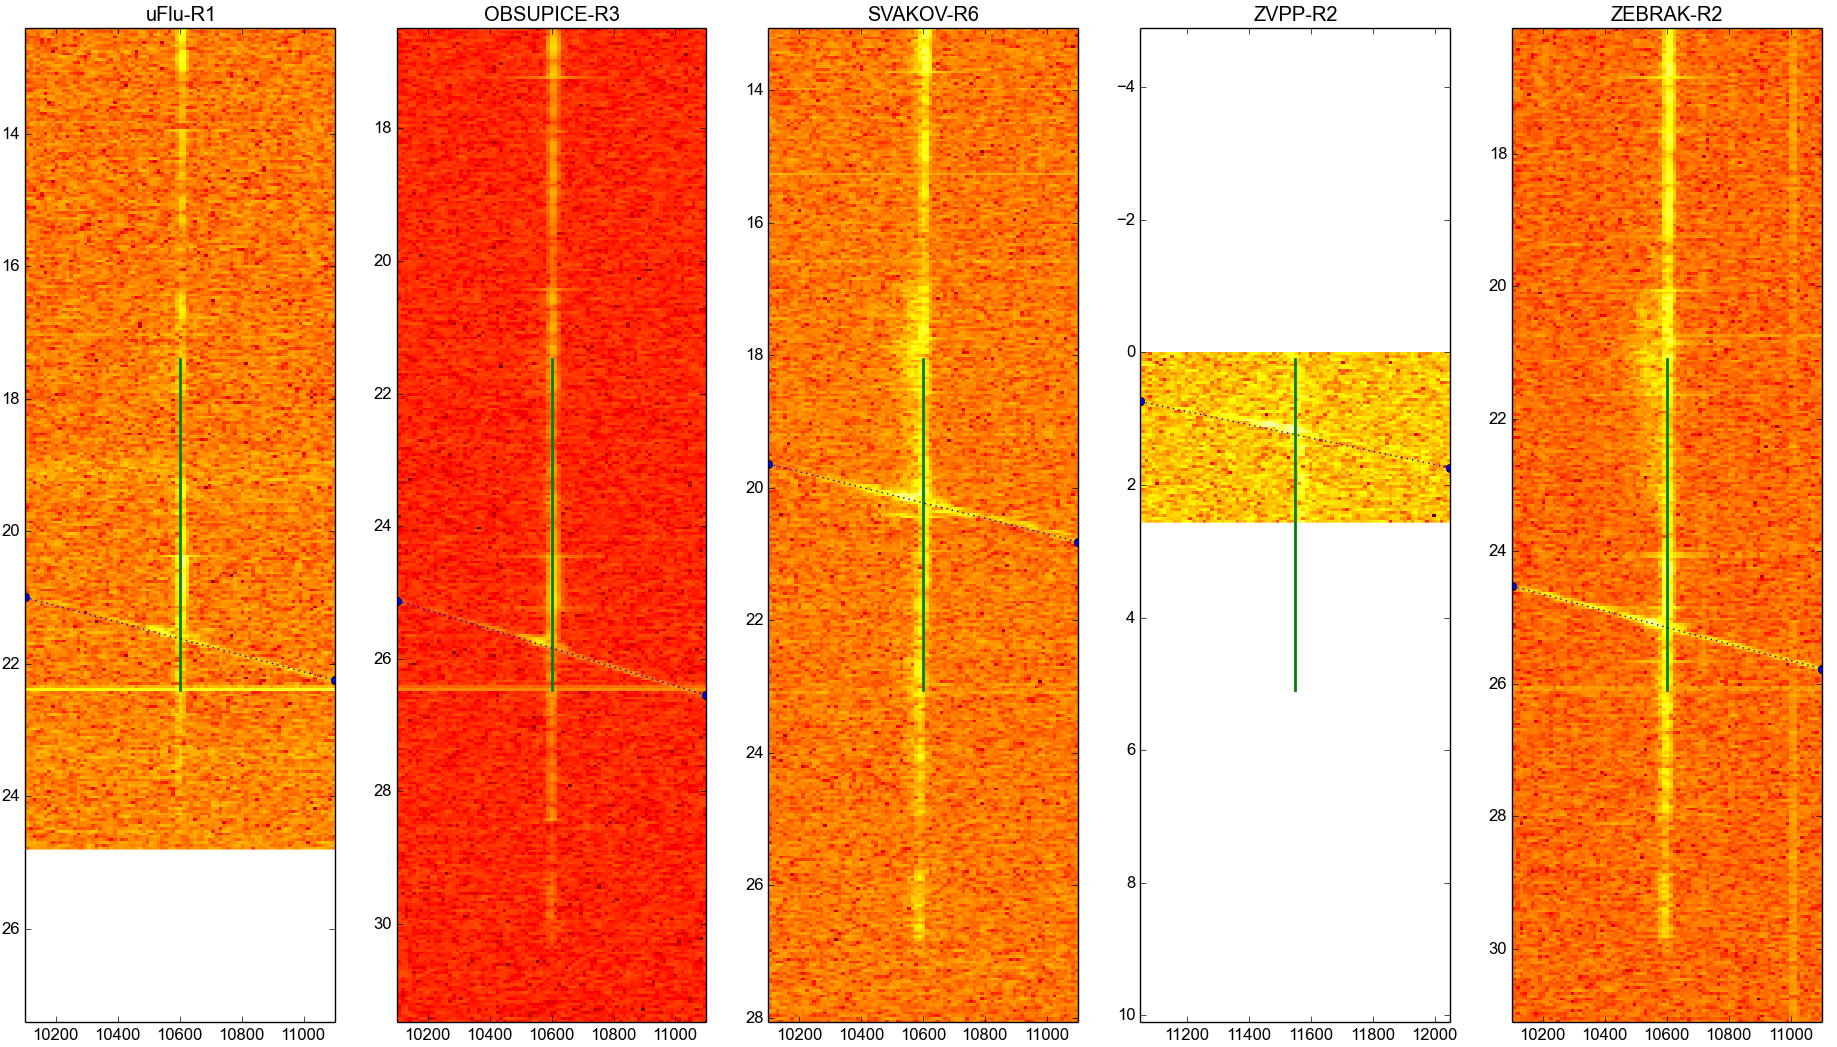
\includegraphics[width=\textwidth]{./img/Raws_analyser.png}
 \caption{Example of meteor reflections for multiple stations - Spectrograms show the time aligned signal evolution over vertical axis. (The oldest data being at the bottom) Horizontal axis corresponds to frequency. (Highest frequency on right)}
  \label{fig:meteor_reflections} 
 \end{center}
\end{figure*}

\begin{equation}
F_{obs} << f_{pe} =\frac{\sqrt{\frac{n_e e^2}{m \epsilon_0}}}{2 \pi}
\label{equ:plasma_frequency}
\end{equation}
\begin{itemize}
\item $n_e$ is the number density of electrons
\item $e$ is the elementary electrical charge
\item $m$ is the effective mass of the electron
\item $\epsilon_0$ is the permittivity of vacuum.
\end{itemize}

Obviously not all parts of the meteor trail are observable from one station as the signal can be scattered to different directions non-specularly.
But if we use multiple receiving stations, we greatly increase the statistical sensitivity because several stations could be located on the reflection spots. Therefore it is very useful to have stations in a form of cooperative detection network.
The network of stations has many advantages over a single transmitter - single receiver configuration. For example it brings robustness which allows operability even in case that a part of the system is under a maintenance and therefore not functional.
                   
There also exist signal processing advantages, especially if we want to compute meteor parameters such as its velocity and trajectory from the meteor radio observation. All physical parameters we could determine from the single reflection are signal intensity and frequency shift in a given time which corresponds to an ionisation intensity and bi-static velocity.
Therefore we must combine information about one meteor event from multiple stations to obtain points in space corresponding to the meteor trajectory. We should alight the events according to time stamps. Therefore, a precise time synchronization between stations is required. The exact required precision depends on the network geometry. But if we want to work in 300 m distance resolution, which is  typical for the current optical methods, we need the time precision on approximately the microseconds scale. Therefore, we needed to develop a high performance receiver with unique parameters, especially with a high quality of time synchronization. Tight time synchronization requirements between nodes increase the complexity of the receiver system. To simplify the development process we used MLAB open source electronic prototyping platform.

As a result a new type of radio meteor detection system is being build, based on a new idea of distributed scientific measurement systems. At the moment Bolidozor network produces large volume of valuable radioastronomy data ready for further processing.  
We currently have a large database of multi-station meteor reflections. Unfortunately, we have yet not reached suitable network geometry to obtain meteor position and trajectory by the known methods \cite{Doppler_method}. 
To overcome this issue, the further evolution of Bolidozor network should be focused on the research of the new trajectory estimation algorithms. We are also working on the network extension with the aim of extension of the service area as well as increasing the stations density. 


\section{VOR Transmitters as signal sources}

For feasibility study of meteor detection based on VOR beacons a numerical signal model has been created. The spectrum of modeled signal is shown in figure \ref{VOR_signal}.

\begin{figure}
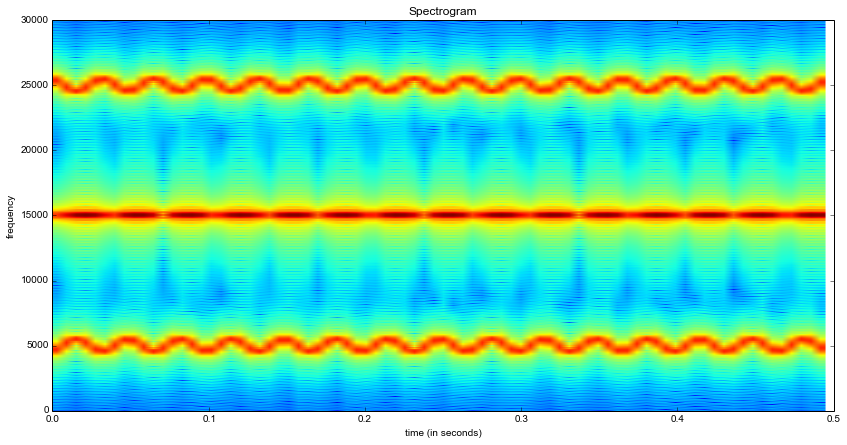
\includegraphics[width=\textwidth]{./img/VOR_signal.png}
\caption{VOR signal numerical model}
\label{VOR_signal}
\end{figure}

This signal is expected to be reflected from meteor ionized trail and signal reflection will be detected and extracted from the noise using the VOR signal replica. An intensity of received reflected signal was modeled by using standard radar equation \ref{Radar_equation}.

\begin{equation}
P_r = \frac{P_t G_t G_r \lambda^2 \sigma}{(4 \pi)^3 R_t ^2 R_r ^2 L}
\label{Radar_equation}
\end{equation}
Where 
\begin{itemize}
\item $P_r$ — Received power in watts.
\item $P_t$ — Peak transmit power in watts.
\item $G_t$ — Transmitter antenna gain.
\item $G_r$ — Receiver antenna gain.
\item $\lambda$ — Radar operating frequency wavelength in meters.
\item $\sigma$ — Target's nonfluctuating radar cross section in square meters.
\item $L$ — General loss factor to account for both system and propagation loss.
\item $R_t$ — Range from the transmitter to the target.
\item $R_r$ — Range from the receiver to the target. 
\end{itemize}

The model generate many meteor trajectories (figure \ref{VOR_meteors} and calculate a power level at receiver for point of closest approach. The resulting power histogram is shown in figure \ref{VOR_meteors_intensity}.

\begin{figure}
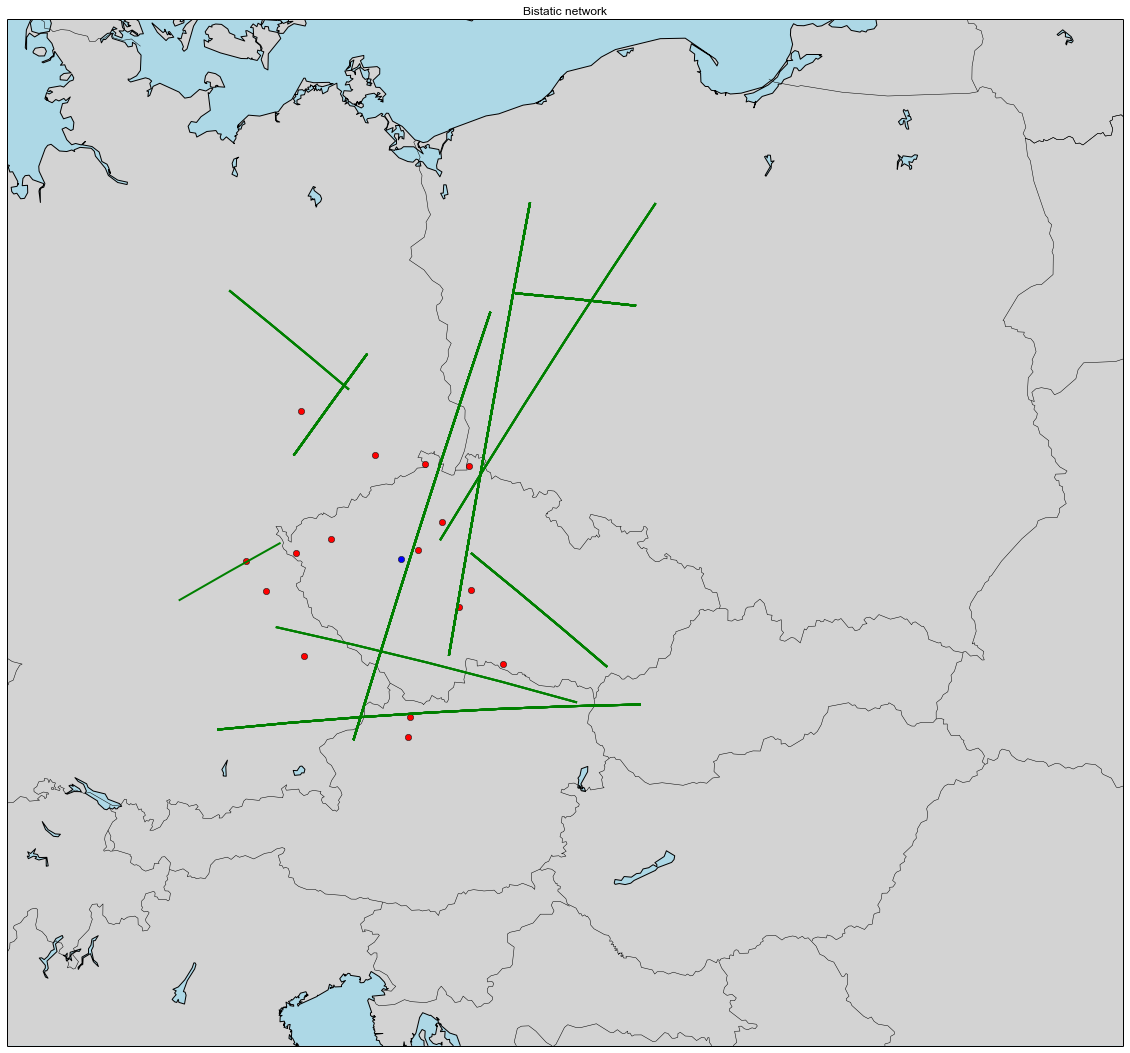
\includegraphics[width=\textwidth]{./img/Modeled_meteor_trajectories.png}
\caption{An examle of random artificial meteor trajectories}
\label{VOR_meteors}
\end{figure}


\begin{figure}
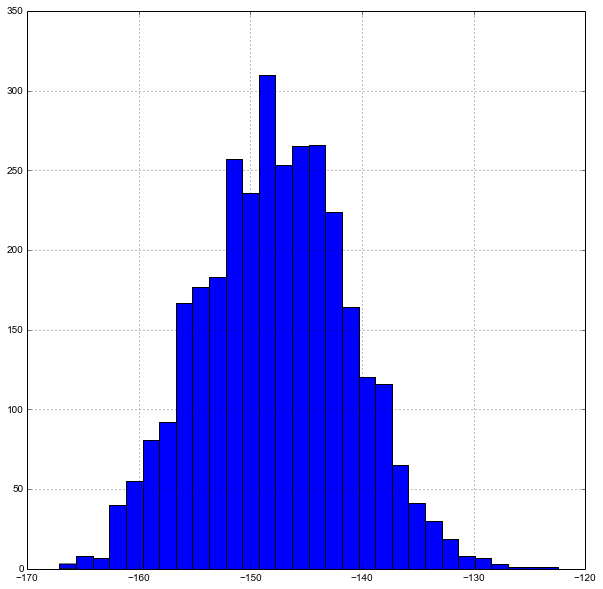
\includegraphics[width=\textwidth]{./img/Meteor_signal_intensity.png}
\caption{Distribution of expected signal power on receiver [dBm] on horizontal axis and meteor count on vertical axis.}
\label{VOR_meteors_intensity}
\end{figure}

\section{Experimental detection of other objects}

\section{Hemispherical radiating pattern antenna design}

A highly directional pattern antenna is usually used for radio meteor observations, but these types of antennas became impractical in cases where we have multiple transmitters spread around a reception station. In that situation the hemispherical sensitivity of  antenna is more important than directional antenna gain. We present a hemispherical radiation pattern antenna design which could be modified for almost any observational frequency reflective by meteor trail. The symmetry of radiation pattern of such antenna allows easy construction of antenna arrays which could be used for angular measurement of received signals.

\subsection{Patch Antenna Design }

Patch antenna was initially examined due to expectation of a simple construction and manufacturing. Antenna was experimentally constructed from wire mesh with  a square grid. This grid was chosen as a compromise between antenna quality (surface conductivity)  and the possibility of icing on antenna’s wire  surfaces. Real prototype of the antenna was made according to the computer model. Unfortunately, after the antenna’s construction and verification it was found that the antenna is very sensitive to deformation of patch base element and for position of the central elevated element. Additionally, the central element must be a precise square to achieve a circular polarization. 

\subsection{Short-circuited quadrifilar helix}

Another antenna type was proposed to overcome the issues of the previous antenna design experiment.  Short-circuited quadrifilar helix (SC-QHA) is a variant of a well known self-phased quadrifilar helix  antenna (SP-QHA). But unlike the SP-QHA type, the  SC-QHA has narrower bandwidth which depends primarily on a bandwidth of a phasing network. Therefore the antenna could be more efficient for narrow band signals like meteor reflections.  The antenna was numerically modeled in NEC2++ software. Source code of  the model is published on github.
Unfortunately the resulting antenna resonance was at 161.5 MHz as is shown in figure 7.

\chapter{Future work}

\section{Meteor signal model improvement}

\section{Expansion of used methods to more objects}


\appendix

\printindex

\appendix

\begin{thebibliography}{99}

\bibliography{refs}
\bibliographystyle{plain}

\bibitem{interplanetary_medium}
MANN, I., PELLINEN-WANNBERG, A., MURAD, E., et. al.
Dusty plasma effects in near earth space and interplanetary medium.
\emph{Space Science Reviews}, 2011, Vol. 161, Issue 1-4: 1-47 
10.1007/s11214-011-9762-3 

\bibitem{Bland01102004}
BLAND, PHILIP, A.,
The Desert Fireball Network
\emph{Astronomy \& Geophysics}, vol. 45, number 5. pages 5.20-5.23
10.1046/j.1468-4004.2003.45520

\bibitem{light_pollution}
KAC, J.,
Meteor Observation and the Light Pollution
\emph{Proceedings of the International Meteor Conference}, Porec, Croatia, 24-27 September, 2009 Edited by Andreic, Z.;  International Meteor Organization, ISBN 2978-2-87355-022-6, pp. 68-75

\bibitem{skiymet}
HOCKINGA, W.K., SINGERB, W., BREMERB, J.,
Meteor radar temperatures at multiple sites derived with SKiYMET radars and compared to OH, rocket and lidar measurements
\emph{Journal of Atmospheric and Solar-Terrestrial Physics}
Volume 66, Issues 6-9, April-June 2004, Pages 585-593
doi:10.1016/j.jastp.2004.01.011

\bibitem{infrasound}
EDWARDS, W. N., BROWN, P. G., WERYK, R. J., et. al.
Infrasonic Observations of Meteoroids: Preliminary Results from a Coordinated Optical-radar-infrasound Observing Campaign
\emph{Earth Moon Planet} (2008) 102:221-229
DOI 10.1007/s11038-007-9154-6

\bibitem{CMOR_radar}
WEBSTER, A. R., BROWN, P. G., JONES, J., et. al.
Canadian Meteor Orbit Radar (CMOR)
\emph{Atmos. Chem. Phys.}, 4, 679-684, 2004
www.atmos-chem-phys.org/acp/4/679/
SRef-ID: 1680-7324/acp/2004-4-679

\bibitem{forward_scatter}
WISLEZ, J.-M.,
Forward scattering of radio waves off meteor trails
\emph{Proceedings of the International Meteor Conference}, Brandenburg, Germany, 1995, p. 99-117

\bibitem{daylight_shover}
CLEGG, J. A. ,HUGHES,  V. A. A., LOVELL, C. B., 
The Daylight Meteor Streams of 1947 May-August
\emph{Monthly Notices of the Royal Astronomical Society}, Vol. 107, p.369

\bibitem{BRAMS}
LAMY, H., ANCIAUX, M., RANVIER, S.,
Recent advances in the BRAMS network
\emph{Proceedings of the International Meteor Conference}, Mistelbach, Austria, 27-30 August 2015, Eds.: Rault, J.-L.; Roggemans, P., International Meteor Organization, ISBN 978-2-87355-029-5, pp. 171-175

\bibitem{Decay_time}
POOLE, L. M. G.,
Duration distribution of radio echoes obtained from underdense shower meteor trains
\emph{Smithsonian Contributions to Astrophysics}, Vol. 11, p.181

\bibitem{GRAVES_radar}
ALLEN, T.,
A GRAVES Sourcebook, Version of 2013-08-07
[Online] Cited 2016-1-23. Available at: http://fas.org/spp/military/program/track/graves.pdf

\bibitem{MLAB}
HORKEL, M., CHROUST, J., JANAS, M., et. al. 
MLAB - The Modular Laboratory project.
[Online] Cited 2016-1-23. Available at: http://www.mlab.cz/

\bibitem{SDR-widget}
STRAND-BERGESEN, B, et. al.
SDR-Widget interface
[Online] Cited 2016-1-23. Available at: https://github.com/borgestrand/sdr-widget

\bibitem{ghpsdr3}
MELTON, J.,
Ghpsdr3
[Online] Cited 2016-1-23. Available at: http://openhpsdr.org/wiki/index.php?title=Ghpsdr3

\bibitem{RMDS}
UNIVERSAL SCIENTIFIC TECHNOLOGIES, s.r.o.,  
Radio meteor detection station RMDS02D
[Online] Cited 2016-1-23. Available at: http://wiki.mlab.cz/doku.php?id=cs:rmds

\bibitem{CAS}
South Bohemian Czech astronomy society department
\emph{Czech astronomy society annual report 2015}
Pages 40-46

\bibitem{iPython}
PEREZ,GRANGER, F.,  BRIAN E.,
IPython: A System for Interactive Scientific Computing
\emph{Computing in Science \& Engineering}
2007, vol 9.,number 3,  Pages 21-29

\bibitem{Jupyter}
RAGAN-KELLEY, M., PEREZ, F., GRANGER, B., et al.,
The Jupyter/IPython architecture: a unified view of computational research, from interactive exploration to communication and publication.
\emph{American Geophysical Union}, Fall Meeting 2014
12/2014

\bibitem{scipy}
JONES E, OLIPHANT E, PETERSON P, et al.
SciPy: Open Source Scientific Tools for Python
2001-, http://www.scipy.org/ [Online; accessed 2016-03-07].

\bibitem{Doppler_method}
STEYAERT, C.,VERBELEN, F., et al.,
Meteor Trajectory from Multiple Station Head Echo Doppler Observations
\emph{WGN, the Journal of the IMO} 38:4 (2010)

\end{thebibliography}

\end{document}